\section{Preliminaries}
In the following, we will provide some background on the \gls{PCS} kinematic model and the derivation of soft robot dynamics following a Lagrangian approach, which are two fundamental topics for this chapter.

\subsection{Piecewise Constant Strain (PCS) Kinematics}\label{sec:pcsregression:pcs_model}
% The continuous nature of soft robots, characterized by their ability to deform over a continuous space, implies that their motion is governed by a set of nonlinear Partial Differential Equations (PDEs)~\citep{gazzola2018forward, della2023model}. 
% As a result, an infinite number of \gls{DOF} are required to accurately characterize their dynamics.
% To make the modeling task tractable,
% , in the first step, the \emph{slender rod} assumption (e.g., Cosserat rods) allows us to describe the behavior of continuum soft robots by considering the deformations of a 1D geometric curve that represents the soft robot's backbone~\citep{gazzola2018forward, della2023model}.
% we apply the \emph{slender rod} assumption (e.g., Cosserat rods) and spatially discretize the backbone curve into $n_\mathrm{s}$ segments of constant strain, which is referred to in the literature as the \gls{DCM}~\citep{gazzola2018forward} theory, or alternatively, \gls{PCS}~\citep{renda2018discrete}.
The \gls{PCS} model~\citep{renda2018discrete} describes the kinematics of continuum soft robots by assuming that the six elemental local backbone strains (shear, axial, bending, twist) are piecewise constant across $n_\mathrm{s}$ segments but variable in time.
We remark that other popular kinematic models for soft robots, such as Piecewise Constant Curvature (PCC)~\citep{webster2010design}, are often times a special case of the \gls{PCS} model.

% To make the modeling task tractable, several assumptions are commonly used. The first one takes advantage of the typical shape of these robots, which tend to have one physical dimension longer than the other two. The analysis of slender, elongated structures can be approximated to its central axis (backbone). The second assumption takes care of the infinite-dimensional problem by approximating the continuous deformation through a space discretization along the backbone. \gls{PCS} models are built upon both of these. The backbone is discretized into a few segments, and the local strains (bending, shear, axial and torsion) are considered constant in space, but variable in time, in each of the segments. Local strains are associated with either a pure translation or rotation along one of the axis of the reference frame attached to the end of a segment. Therefore, an analogy can be drawn between joint states in rigid robots and local strains in continuum robots: just like the pose of a rigid link is dependent on the previous joint variables, the pose at a certain point of the soft robot is dependent on the local strains of all the previous segments.   %At the end of each segment is attached a reference frame $\{S_i\}$ and its configuration is defined relative to the frame of the previous one, $\{S_{i-1}\}$.

For the planar case, the configuration of the $i$th segment is referred to as
\begin{equation}
    q_i= \begin{bmatrix}
    \kappa_{\mathrm{be},i} & \sigma_{\mathrm{sh},i} & \sigma_{\mathrm{ax},i}
\end{bmatrix}^\top \in \mathbb{R}^3,
\end{equation}
where $\kappa_{\mathrm{be},i}, \sigma_{\mathrm{sh},i}, \sigma_{\mathrm{ax},i}$ are the bending, shear, and axial strains, respectively, and $i \in \{1, \dots, n_\mathrm{s} \}$. 
Therefore, the configuration of the entire soft robot is defined as $q \in \mathbb{R}^{n_\mathrm{q}}$, where $n_\mathrm{q} = 3 n_\mathrm{s}$.
We also have access to closed-form expressions for the forward and inverse kinematics of a single constant strain segment~\citep{stolzle2024experimental}.
As a consequence, forward and inverse kinematics for the entire planar \gls{PCS} soft robot can be implemented using an iterative procedure starting at the proximal end without having to resort to differential (inverse) kinematic techniques.
Namely, the forward kinematics $\pi: \mathbb{R}^{n_\mathrm{q}} \to SE(2)$ allow us to compute the pose $\chi_j = \begin{bmatrix}
    p_{\mathrm{x},j} & p_{\mathrm{y},j} & \theta_j
\end{bmatrix}^\top = \vartheta(q,s_j)$, where $s_j \in [0, L]$ is the backbone abscissa/coordinate, $L$ is the length of the entire continuum structure in an undeformed configuration, $p_{\mathrm{x},j}, p_{\mathrm{y},j} \in \mathbb{R}$ and $\theta_j$ are the positions and orientations at point $s$, respectively.
Given $N$ poses along the backbone, we can also define the inverse kinematic mapping $\varrho: 3N \times N \to n_\mathrm{q}$ that provides us with the configuration $q = \varrho(\chi, s)$ in closed-form. Here, $q_i$ will describe the configuration of the $i$th constant strain segment connecting the $i-1$th and the $i$th markers with associated poses $\chi_{i-1}$ and $\chi_i$. This means that $n_\mathrm{s} = N -1$ in order that $\rho$ can be bijective.


% \begin{figure}[htbp]
% \centerline{\includegraphics[scale=.5]{figures/pcs_diagram_2.png}}
% \caption{Illustration of a planar \gls{PCS} segment. In light gray the segment is represented only undergoing bending deformation, with amplitude $\theta_i$. In blue, the same segment also exhibits shear and axial displacements. ${S_i}$ and ${S_{i-1}}$ denote the local frames of the current and preceding segments, respectively. $\delta L_i$ and $\delta x_i$ indicate the displacements caused by shear and axial strains.}
% \label{fig:pcsregression:pcs_diagram}
% \end{figure}

% \subsubsection{Forward Kinematics}
% Subsequently, we can leverage to kinematic model to determine the homogeneous transformation $T_{i-1}^{i}(q_i) \in SE(2)$ between the proximal and the distal segment of the $i$th segment~\citep{stolzle2024experimental}
% \begin{equation}
% \begin{split}
%     T_{i-1}^{i} =& \: \begin{bmatrix}
%         \cos \left ( \theta_{i-1}^{i} \right ) & -\sin \left ( \theta_{i-1}^{i} \right ) & p_{\mathrm{x},i-1}^{i}\\
%         \sin \left ( \theta_{i-1}^{i} \right ) & \cos \left ( \theta_{i-1}^{i} \right ) & p_{\mathrm{y},i-1}^{i}\\
%         0 & 0 & 1
%     \end{bmatrix},\\
%     p_{\mathrm{x},i-1}^{i} =& \: \sigma_{\mathrm{sh},i} \frac{\sin \left ( \theta_{i-1}^{i} \right )}{\kappa_{\mathrm{be},i}} + \sigma_{\mathrm{ax},i} \, \frac{\cos \left ( \theta_{i-1}^{i} \right ) - 1}{\kappa_{\mathrm{be},i}}\\
%     p_{\mathrm{y},i-1}^{i} =& \: \sigma_{\mathrm{sh},i} \frac{1 - \cos \left ( \theta_{i-1}^{i} \right )}{\kappa_{\mathrm{be},i}} + \sigma_{\mathrm{ax},i} \, \frac{\sin \left ( \theta_{i-1}^{i} \right )}{\kappa_{\mathrm{be},i}}\\
%     \theta_{i-1}^{i} =& \: \kappa_\mathrm{be} \, L_i
% \end{split}
% \end{equation}
% where $L_i \in \mathbb{R}_{>0}$ is the segment's length and $\chi_{i-1}^{i} = \begin{bmatrix}
%     p_{\mathrm{x},i-1}^{i} & p_{\mathrm{y},i-1}^{i} & \theta_{i-1}^{i}
% \end{bmatrix}^\top \in \mathbb{R}^3$ is the pose of the distal tip in the local frame of the proximal end of the segment: $p_{x},p_{y} \in \mathbb{R}$ refer to the x- and y-position, respectively, and $\theta \in \mathbb{R}$ denotes the orientation.
% Here, we assume that the distal end of the $i-1$th segment coincides with the proximal end of the $i$th segment. In the following, we will refer to $\chi_i \in \mathbb{R}^3$ as the pose of the tip of the $i$th segment in inertial coordinates which can be computed iteratively using the robot's forward kinematics $\vartheta_i: \mathbb{R}^{3i} \to \mathbb{R}^3$ as $\chi_i = \chi_0^{i} = \vartheta_i(q_{1:i})$, where $q_{1:i}$ are the concatenated configurations of the first $i$ segments and the corresponding homogeneous transformation from the base of the robot to the tip of the $i$th segment is given as $T_{0}^i = \Vartheta_{j=1}^{i} T_{j-1}^{j}(q_j)$.

% \subsubsection{Inverse Kinematics}
% Assuming that the pose of the distal end of each segment is known, also a closed-form solution to the inverse kinematics exists~\citep{stolzle2024experimental}, in which the configuration of each segment is iteratively determined as

% \begin{equation}
% \begin{split}
%     q_i = \varrho_i(\chi_0^i, q_{1:i-1}) = \frac{\theta_{i-1}^i}{2 \, L_i} \begin{bmatrix}
%         2\\
%         p_{\mathrm{x},i-1}^{i} - \frac{p_{\mathrm{x},i-1}^{i} \sin \left (\theta_{i-1}^i \right )}{\cos \left (\theta_{i-1}^i \right ) - 1}\\
%         -p_{\mathrm{y},i-1}^{i} - \frac{p_{\mathrm{y},i-1}^{i} \sin \left (\theta_{i-1}^i \right )}{\cos \left (\theta_{i-1}^i \right ) - 1}
%     \end{bmatrix},\\
%     T_{i-1}^{i} = T(\chi_0^i) \, T(\vartheta_{i-1}(q_{1:i-1}))
% \end{split}
% \end{equation}
% starting with the most proximal segment (i.e., $i=1$). 
% We denote with the operation \textcolor{red}{TODO}
% Here, $\varrho_i: \mathbb{R}^3 \times $ describes the inverse kinematics that identifies the configuration of the $i$th segment as a function of the inertial pose of the tip of the $i$th segment $\chi_0^i$ and the configuration of the more proximal segments $q_{1:i-1} \in \mathbb{R}^{3(i-1)}$.

% This configuration vector fully specifies the shape of the robot. Given $s \in [0,L_{0,i}]$ the coordinate along the backbone, the angle of the central axis along the segment $i$ can be determined by integration of the curvature \citep{webster2010design} via 
% \begin{align}
%     \theta_i = \int_{0}^{s} \kappa_{\text{be},i} \,dv = \kappa_{\text{be},i} s \,.
% \end{align}
% The segment's position $[p_{x,i},p_{y,i}]$ can be calculated by integrating the shear and axial strains (properly rotated) 
% \begin{align}
%     \begin{bmatrix}
%         p_{x,i}\\
%         p_{y,i}
%     \end{bmatrix} =
%     \int_{0}^{s} \begin{bmatrix}
%         \cos{\theta_i} & -\sin{\theta_i} \\
%         \sin{\theta_i} & \cos{\theta_i}
%     \end{bmatrix} \begin{bmatrix}
%         \sigma_{\text{sh},i} \\
%         1 + \sigma_{\text{ax},i}
%     \end{bmatrix} \,dv .
% \end{align}

% Knowing the above relations, the forward and inverse kinematics relating the segment's pose $\chi_i=[p_{x,i},p_{y,i},\theta_i]$ and configuration $q_i$ can be written in closed form \citep{stolzle2024experimental} as
% \begin{align} 
%     \chi_i=\begin{bmatrix}
%         p_{x,i}\\
%         p_{y,i}\\
%         \theta_i
%     \end{bmatrix}=\begin{bmatrix}
%         \sigma_{\text{sh},i} \frac{\sin({\kappa_{\text{be},i} s})}{\kappa_{\text{be},i}} + (1+\sigma_{\text{ax},i}) \frac{\cos({\kappa_{\text{be},i} s}) - 1}{\kappa_{\text{be},i}} \\
%         \sigma_{\text{sh},i} \frac{1 - \cos({\kappa_{\text{be},i}s})}{\kappa_{\text{be},i}} + (1+\sigma_{\text{ax},i}) \frac{\sin({\kappa_{\text{be},i}s})}{\kappa_{\text{be},i}} \\
%         \kappa_{\text{be},i}s
%     \end{bmatrix} ,
%     \label{eq:pcsregression:pcsregression:forward_kin_pcs}
% \end{align}
% and 
% \begin{align}
%     q_i=\begin{bmatrix}
%         \theta_i / s \\
%         \theta_i \left(p_{y,i} - \frac{p_{x,i}\sin{(\theta_i)}}{\cos{(\theta_i)}-1} \right) / 2s \\
%         -1+\theta_i \left(-p_{x,i} - \frac{p_{y,i}\sin{(\theta_i)}}{\cos{(\theta_i)}-1} \right) / 2s
%     \end{bmatrix} ,
%     \label{eq:pcsregression:inverse_kin_pcs}
% \end{align}
% respectively. Notice that \eqref{eq:pcsregression:forward_kin_pcs} and \eqref{eq:pcsregression:inverse_kin_pcs} have no singularity for $\kappa_{\text{be},i} = 0$ and $\theta_i=0$. The limit in this situation where no curvature occurs in the segment is well defined and is equal to $\begin{bmatrix}
%     \sigma_{sh} s & (1+\sigma_{ax})s & 0
% \end{bmatrix}^{\top}$ and $\begin{bmatrix}
%     0 & p_{x,i}/s & -1+p_{y,i}/s
% \end{bmatrix}^{\top}$, respectively. However, some numerical instabilities might arise in practice \citep{della2023model}. 

\subsection{Lagrangian Dynamics}\label{sub:pcsregression:lagr_dynamics}
The Lagrangian of a mechanical system as a function of the configuration $q \in \mathbb{R}^{n_\mathrm{q}}$ and the corresponding time derivative $\dot{q} \in \mathbb{R}^{n_\mathrm{q}}$ can be expressed as
\begin{equation}
    \mathcal{L}(q, \dot{q}) = \mathcal{T}(q, \dot{q}) - \mathcal{U}(q) = \underbrace{\frac{1}{2}\dot{q}^\top \, M(q) \, \dot{q}}_{\mathcal{T}(q, \dot{q})} - \underbrace{\frac{1}{2} q^\top K q - \int G(q) \: \mathrm{d}q}_{\mathcal{U}(q)},
\end{equation}
where $\mathcal{T}(q, \dot{q})$, $\mathcal{U}(q)$ are the kinetic and potential energy of the system, respectively, and $M(q) \succ 0 \in \mathbb{R}^{n_\mathrm{q} \times n_\mathrm{q}}$ is referred to as the mass matrix. $G(q) \in \mathbb{R}^{n_\mathrm{q}}$ contribute the gravitational forces and $K \in \mathbb{R}^{n_\mathrm{q} \times n_\mathrm{q}}$ represents the linear elastic stiffness of the system.
Subsequently, the Euler-Lagrangian equation can be leveraged to derive the \gls{EOM} of continuum soft robots as~\citep{della2023model, liu2024physics}
\begin{equation}
    \diffp[2]{\mathcal{L}}{{\dot{q}}}\ddot{q} + \diffp{\mathcal{L}}{{q}{\dot{q}}}\dot{q} - \diffp{\mathcal{L}}{{q}} + D\dot{q} = \tau
\end{equation}
where we are also considering the generalized dissipative forces $D\dot{q}$ and the actuation torques $\tau \in \mathbb{R}^{n_\mathrm{q}}$. 
In this work, we assume, without loss of generality, that both the stiffness matrix $K = \mathrm{diag}(k_1, \dots, k_{n_\mathrm{q}})$ and the damping matrix $D = \mathrm{diag}(d_1, \dots, d_{n_\mathrm{q}}) \succeq 0$ are diagonal.

\begin{figure}[ht]
    \center
    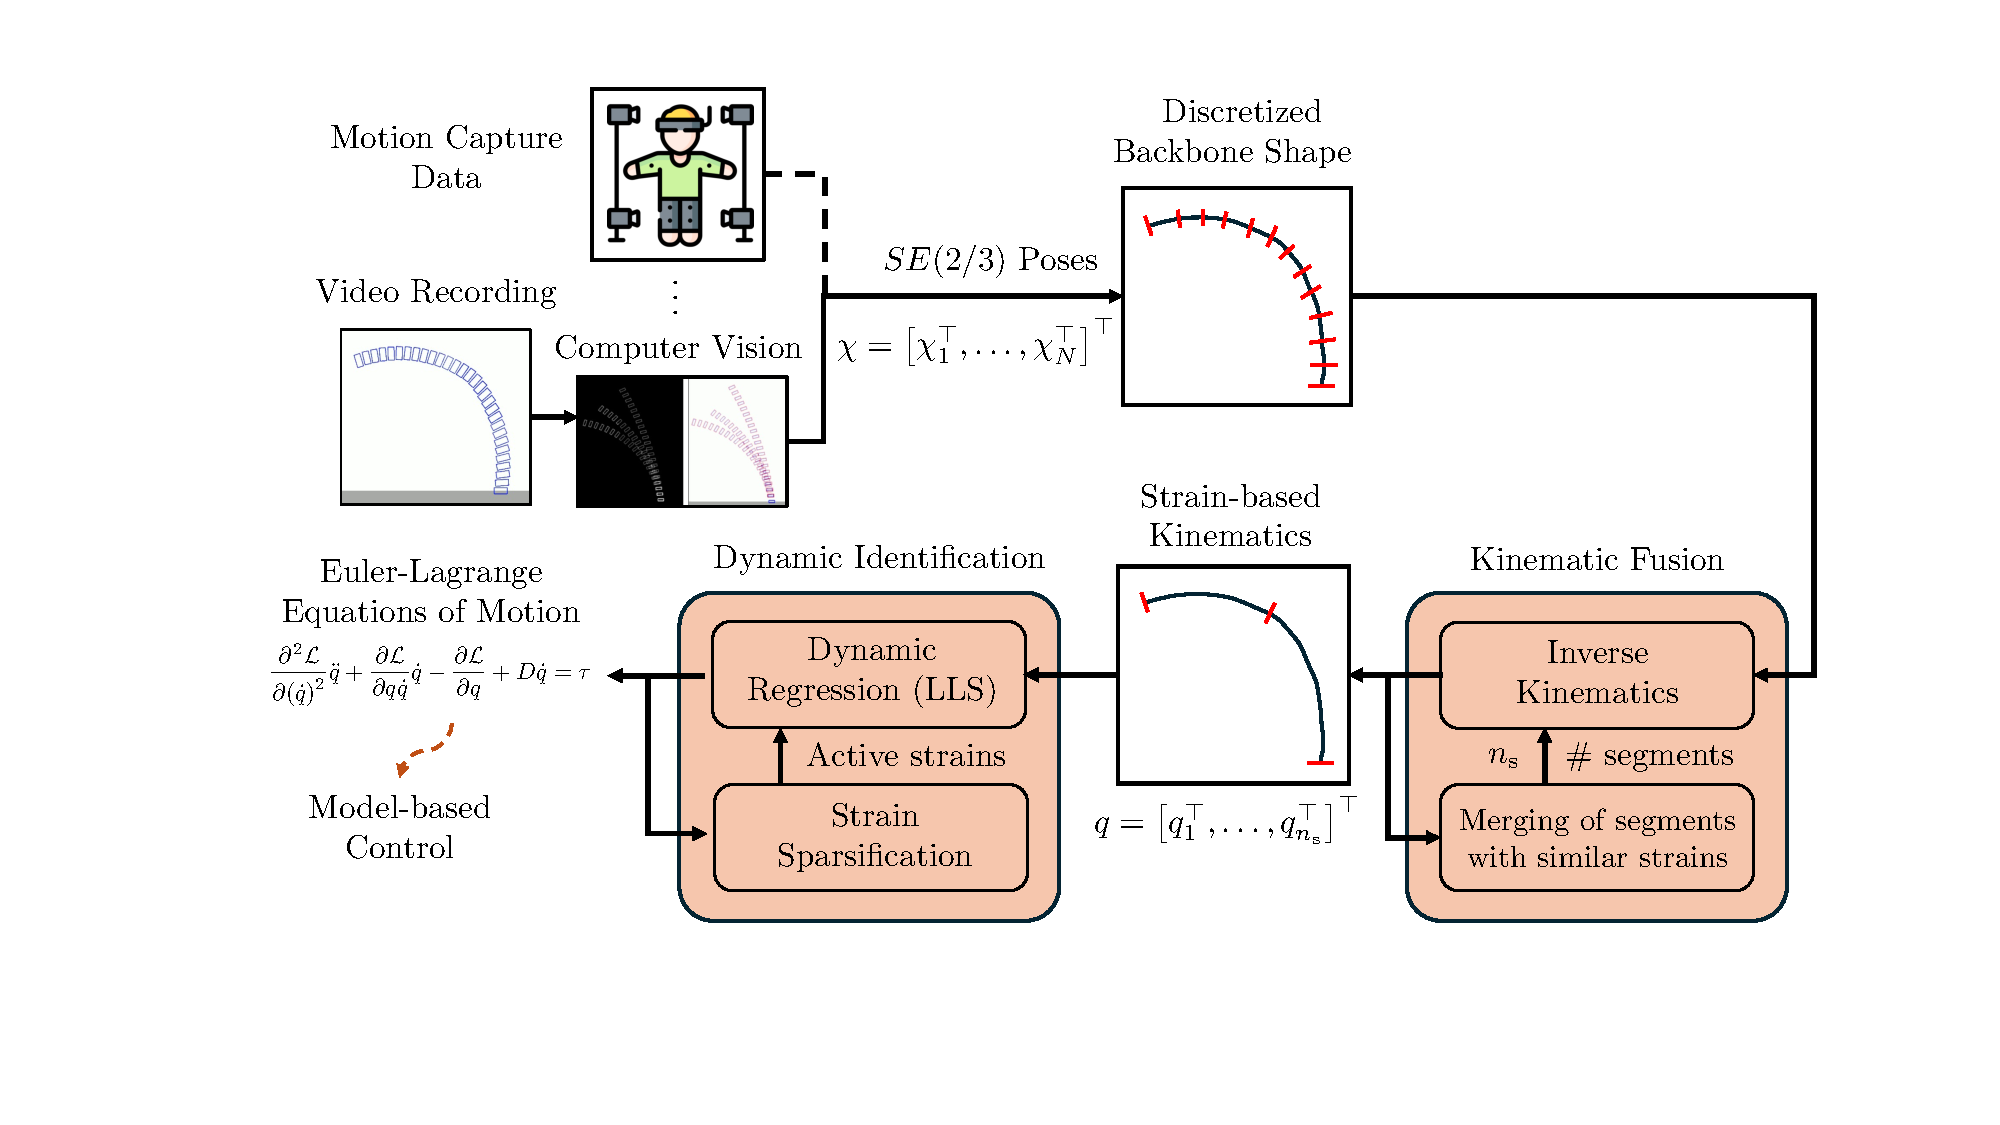
\includegraphics[width=0.9\textwidth]{pcsregression/figures/pcs_regression_overview_v2_cropped.pdf}
    \caption{
        Overview of the proposed methodology with the key contributions (\emph{Kinematic Fusion} and \emph{Dynamic Regression and Strain Sparsification}) highlighted in orange. 
        \textbf{Inputs:} We consider $N$ Cartesian pose measurements $\chi$ distributed along the soft robot backbone, for example, obtained using Computer Vision (CV) techniques from video recordings, as inputs.
        \textbf{Kinematic Fusion:} We apply an iterative procedure that involves (i) computing the robot configuration $q$ using \gls{PCS} inverse kinematics, and (ii), to avoid overly complex and high-dimensional models, we merge adjacent segments with similar strains across the dataset into one segment of constant strain.
        \textbf{Dynamic Regression:} We identify the PCS dynamic model by iteratively regressing coefficients using linear least squares and further reduce the model complexity by neglecting insignificant strains.
        \textbf{Output:} The identified dynamic model has a Lagrangian structure suitable, for example, for model-based control applications.
    }
    \label{fig:pcsregression:overall_diag}
\end{figure}

% The dynamics of a soft robot, irrespective of the kinematic model that is chosen, can be expressed in Euler-Lagrangian fashion as a function of the configuration $q \in \mathbb{R}^{n_\mathrm{q}}$ and the corresponding time derivative $\dot{q} \in \mathbb{R}^{n_\mathrm{q}}$~\citep{della2023model}
% \begin{equation}
%     M(q) \, \ddot{q} + C(q, \dot{q}) \, \dot{q} + G(q) + K q + Dq = A(q),
% \end{equation}
% where $M \in $

% The dynamics of physical systems are commonly expressed using the Lagrangian mechanics. According to this, an $n_\mathrm{q}$-DOF system can be described by a set of generalized coordinates $q \in \mathbb{R}^{n_\mathrm{q}}$, their velocities $\dot{q} \in \mathbb{R}^{n_\mathrm{q}}$, and a scalar quantity known as the Lagrangian, expressed as
% \begin{align}
%     \mathcal{L}(q, \dot{q}) = \mathcal{T}(q, \dot{q}) - \mathcal{U}(q).
% \end{align}
% The kinetic energy is given by $\mathcal{T}(q, \dot{q}) = \frac{1}{2}\dot{q}^\top \, M(q) \, \dot{q}$, with $M(q) \succ 0 \in \mathbb{R}^{n_\mathrm{q} \times n_\mathrm{q}}$ being referred to as the mass matrix. The potential energy $\mathcal{U}(q)$ includes the gravitational and elastic potential. % $V(q) = V_G(q) + V_K(q)$. % and $V_K(q) = \frac{1}{2}q^\intercal K q$ is the elastic potential, with $K \in \mathbb{R}^{n\times n}$ being the stiffness matrix. 
% Applying the principle of least action to the Lagrangian yields the Euler-Lagrangian equations which express the \gls{EOM} as
% \begin{align}\label{eq:pcsregression:euler-lagrange}
%     \diff{}{t}\left( \diffp{\mathcal{L}(q,\dot{q})}{{\dot{q}}} \right) - \diffp{\mathcal{L}(q,\dot{q})}{{q}} = F_{\text{ext}} \,,
% \end{align}
% where $F_{\text{ext}} \in \mathbb{R}^n$ represents all non-conservative forces. We here consider external forces to be restricted to velocity-dependent dissipative forces $F_{d} \in \mathbb{R}^n$ and actuation forces $F_a \in \mathbb{R}^n$, which generally are given by
% \begin{align}
%     F_{\text{ext}} = F_d+F_{a}=-D(q)\dot{q} + A(q)\tau \,,
% \end{align}
% where $D(q) \in \mathbb{R}^{n\times n}$ is the damping matrix and $A(q)\tau$ represent the actuator forces applied on the robot. $\tau \in \mathbb{R}^m$ is the control input and $A(q) \in \mathbb{R}^{n\times m}$ is the matrix that maps the point of application of the actuation to the configuration space. In this work, we will assume that $D$ is diagonal and constant and that actuators are directly collocated on the configurations, resulting in $\tau\in \mathbb{R}^n$ and $A(q)$ being the identity matrix.

% By expanding \eqref{eq:pcsregression:euler-lagrange} and after some manipulation, this set of equations can be rearranged into a more convenient matrix form,
% \begin{align}
%     M(q)\ddot{q} + C(q,\dot{q})\dot{q} + G(q) + Kq + D\dot{q} = \tau\,.
% \end{align}
% Here, $C(q,\dot{q})\dot{q} \in \mathbb{R}^n$ represents the Coriolis and centrifugal force contribution, while $G(q) \in \mathbb{R}^n$ and $Kq$ denote the gravitational and elastic actions, where $K \in \mathbb{R}^{n\times n}$ is the diagonal stiffness matrix.
% % \begin{align}
% %     G(q)=\diffp{V_G}{{q}} ,\,\, K(q)=\diffp{V_K}{{q}} .
% %\end{align}

% This dynamic formulation can be derived for a \gls{PCS} soft robot parametrization by combining its kinematic model with the inertial and impedance properties of its structure. The details for the derivations of each of these terms can be found in \citep{della2023model}.%Appendix \ref{ap:dynamics_pcs}.

% \begin{figure*}[ht]
%     \center
%     \subfigure[Kinematic Fusion Scheme]{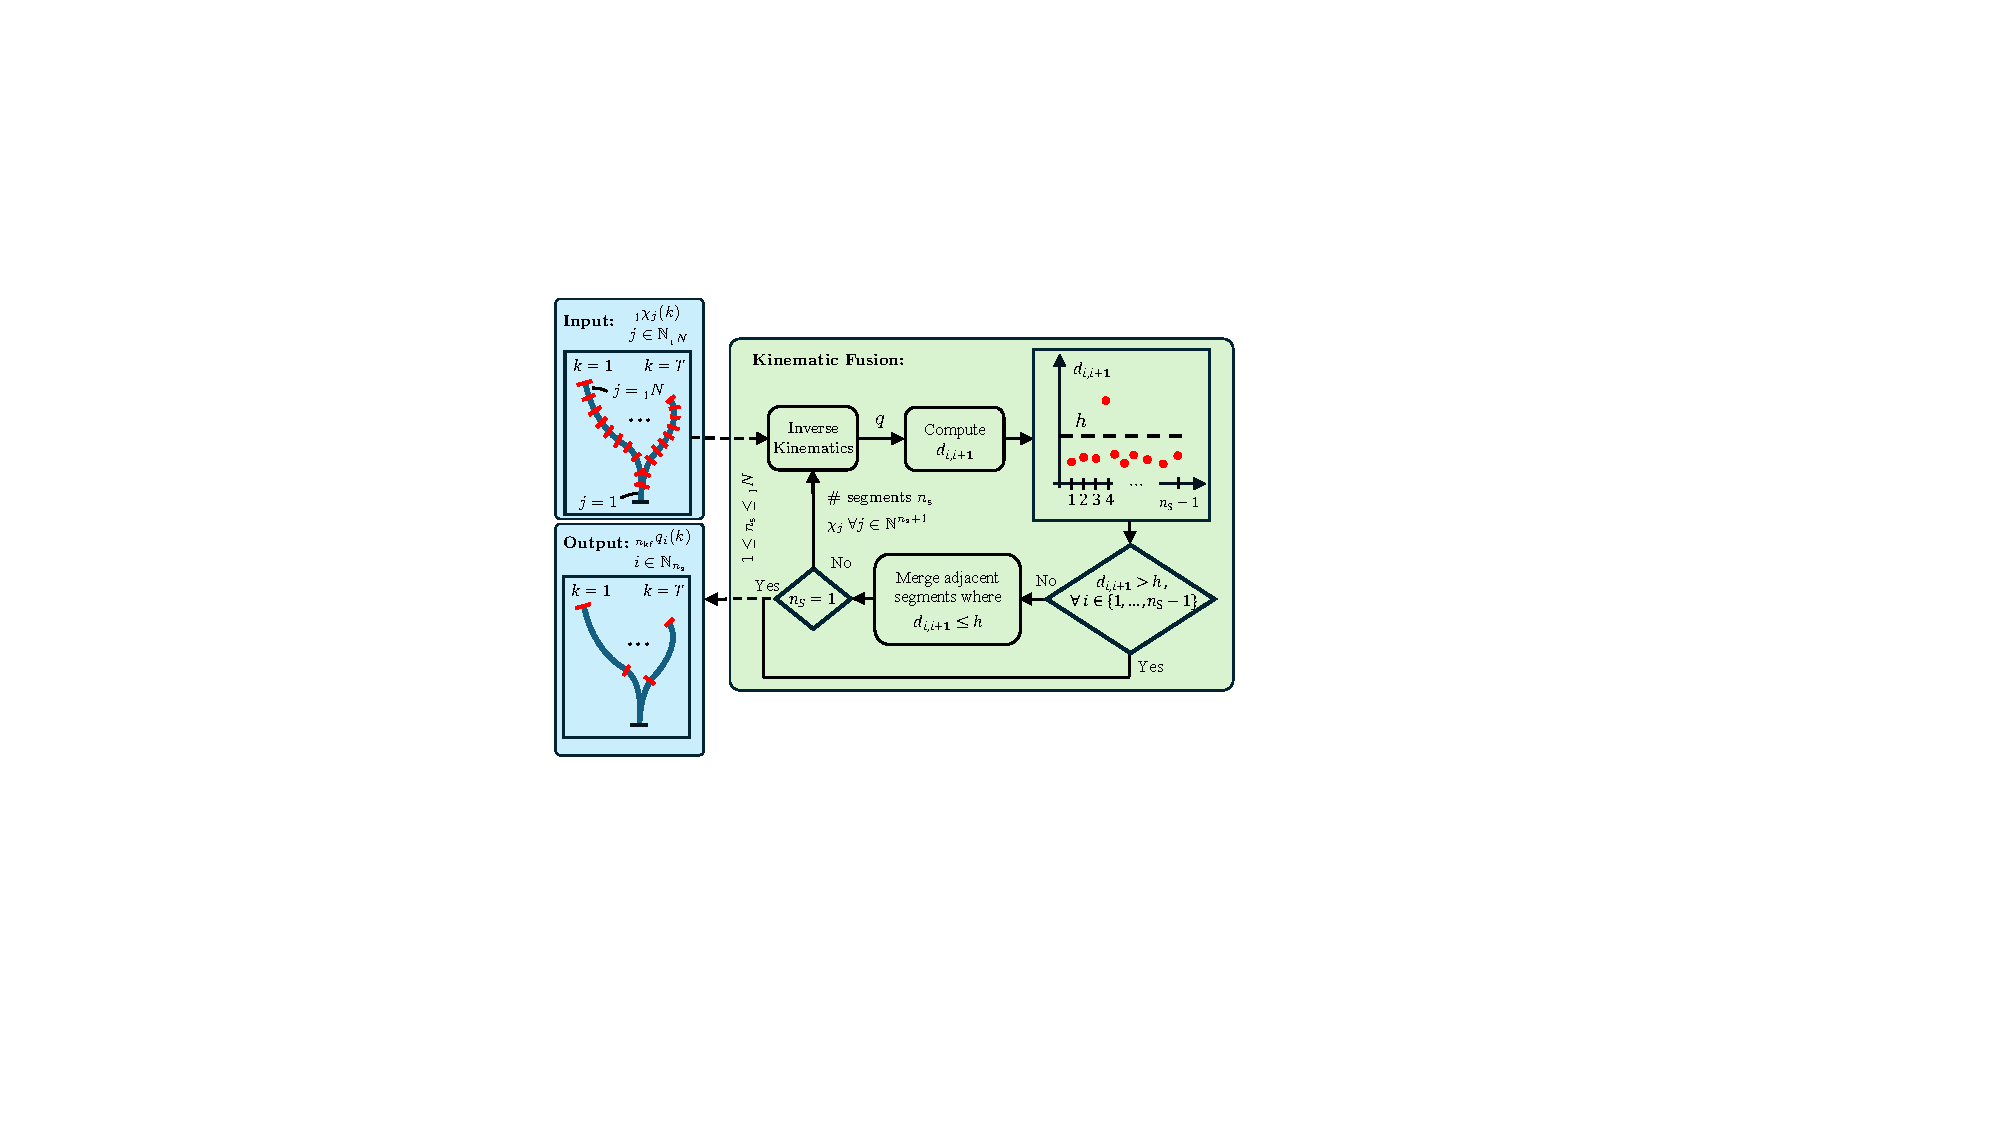
\includegraphics[width=0.34\textwidth]{pcsregression/figures/diagram_kinematic_fusion_v3_cropped.pdf}\label{fig:pcsregression:kin_regr}}
%     \hfill
%     \subfigure[Dynamic Regression \& Strain Sparsification Scheme]{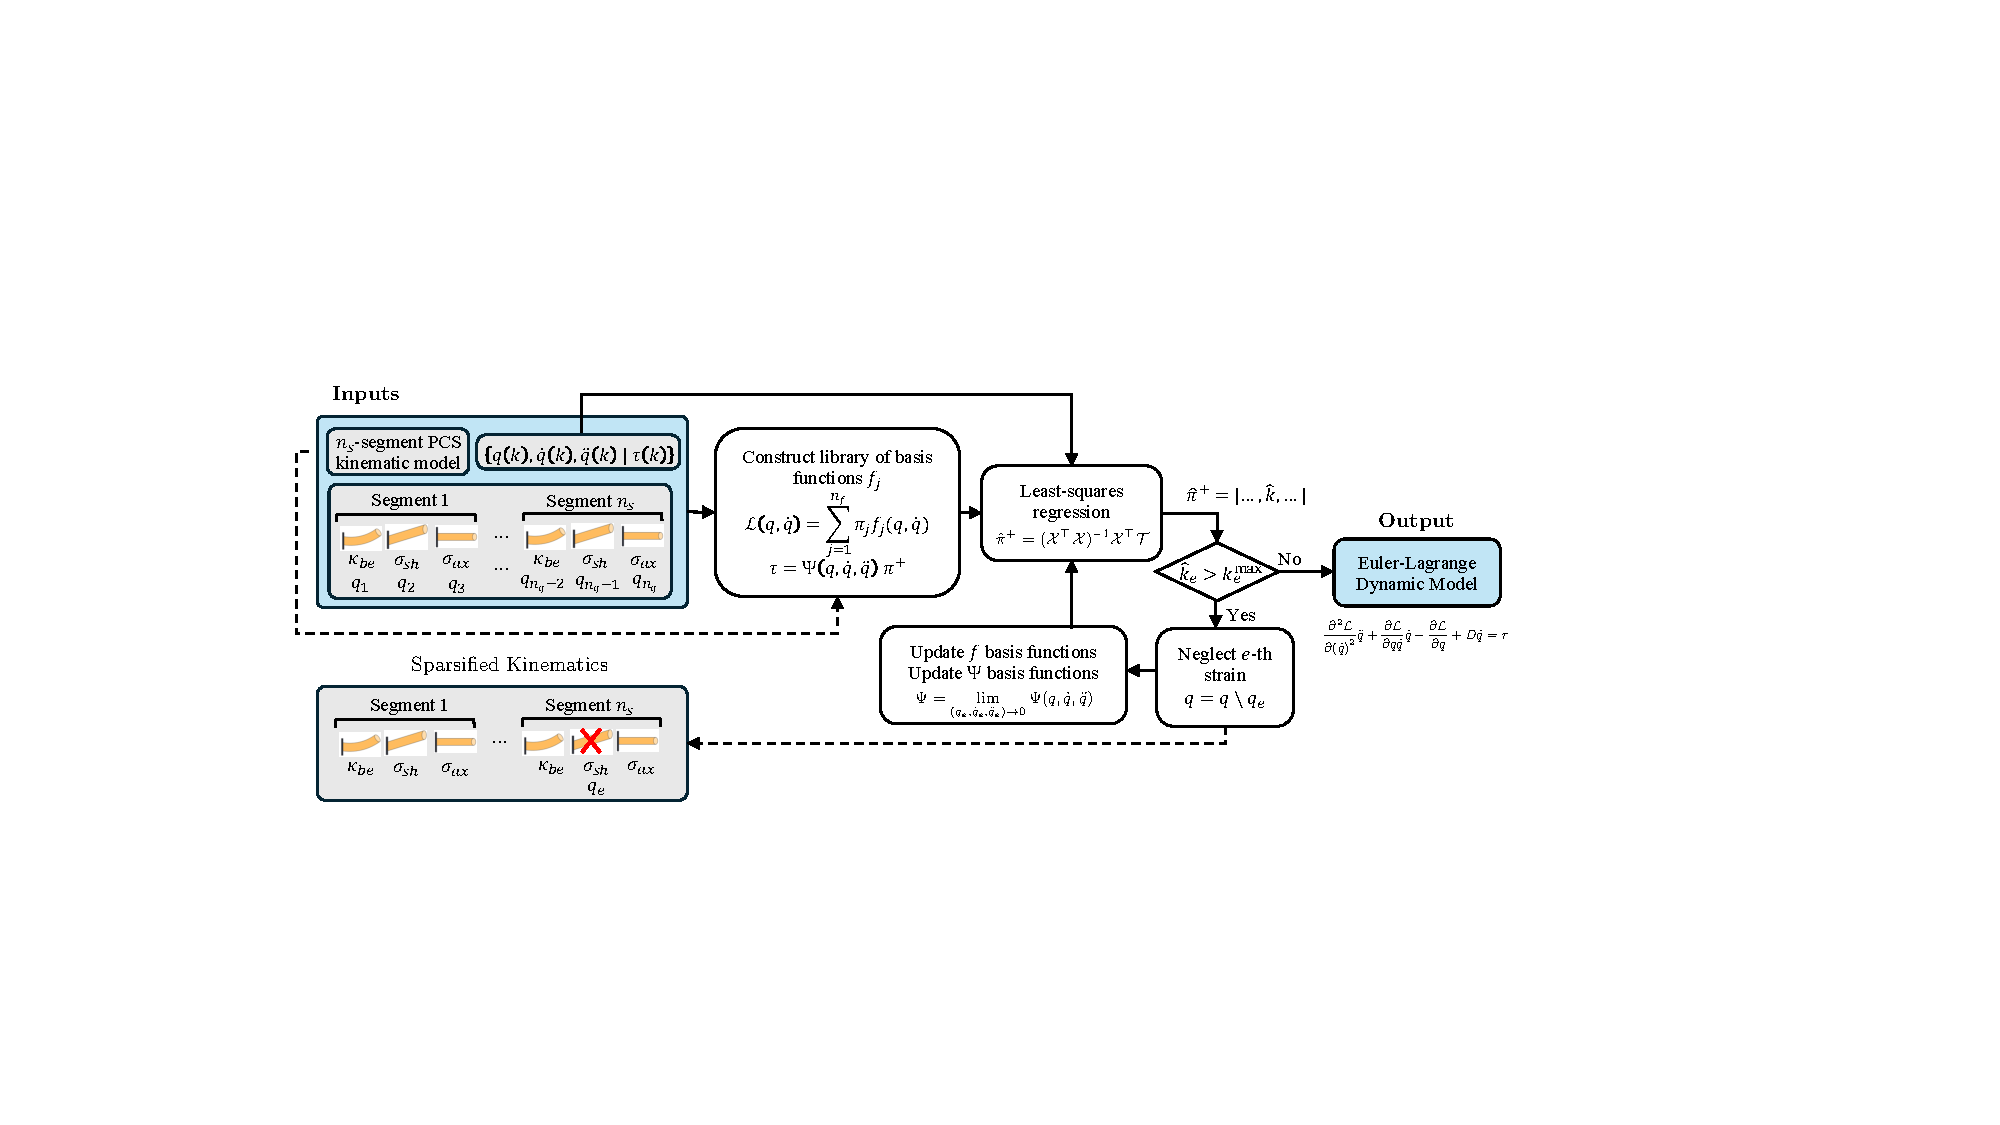
\includegraphics[width=0.65\textwidth]{pcsregression/figures/diagram_dynamic_regression_v2_cropped.pdf}\label{fig:pcsregression:dyn_regr}}
%     \caption{\textbf{Panel (a):} Schematic of the kinematic fusion algorithm. As inputs serve a sequence of $N$ discrete poses along the backbone of the soft robot. Next, we execute inverse kinematics in closed form with a $n_\mathrm{s} = N-1$ segment \gls{PCS} model to identify the (unmerged) configuration of the robot. Initially, each constant strain segment connects two neighboring backbone poses. Subsequently, we compute a strain similarity measure $\bar{d}_{i,i+1}$ between each pair of adjacent segments. If segments exhibit a similar strain (i.e., the metric falls below a threshold $h$), we merge them into one constant strain segment. This process is repeated until no more merging is possible, resulting in a kinematic model with (hopefully) fewer segments: $1 \leq n_\mathrm{s} \leq N-1$. 
%     \textbf{Panel (b):} Schematic of the dynamic model identification process that simultaneously regresses the dynamic parameters and neglects unimportant strains. Based on a $n_\mathrm{s}$-segment PCS model, a library of basis functions is constructed to parameterize the system’s Lagrangian and \gls{EOM}. A regression framework is established on a dataset of configuration-space positions $\dot{q}(k)$, velocities $\dot{q}(k)$, accelerations $\ddot{q}(k)$, and actuation torques $\tau(k)$ that estimates the dynamic parameters $\hat{\pi}^+$ with closed-form, linear least squares. Strains that exhibit a stiffness higher than a predefined threshold are neglected, prompting adjustments to the basis functions. Subsequently, this procedure is repeated until all strain stiffnesses lie below the threshold.}
% \end{figure*}